\documentclass[a4paper]{article}
\usepackage[margin=2cm]{geometry}
\usepackage{graphicx}
\usepackage{enumitem}
\setlist[description]{}

\begin{document}

\title{Torneos de Yu-Gi-Oh}
\author{
  \begin{tabular}{c}
    Chavely 02110766835 \\
    Jos\'e Carlos CI \\
    L\'azaro David CI \\
    Max CI
  \end{tabular}
}
\date{\today}
\maketitle
\newpage

\section{Objetivos del producto}
Este sistema permitirá a los organizadores de torneos crear, administrar y seguir el progreso de torneos de
Yu-Gi-Oh!, ası́ como proporcionar a los jugadores una plataforma para registrarse en estos eventos y consultar
estadı́sticas relevantes.

\newpage

\section{Requerimientos tecnicos}
\

\section{Forma de instalar la aplicaci\'on}
\begin{enumerate}
\item Abrir una consola
\item Colocarse en la carpeta ra\'iz del proyecto(YuGiOh)
\item escribir "dotnet run"
\end{enumerate}

\newpage
\section{Modelo conceptual de la base de datos:}
\begin{figure}[h]
  \centering
  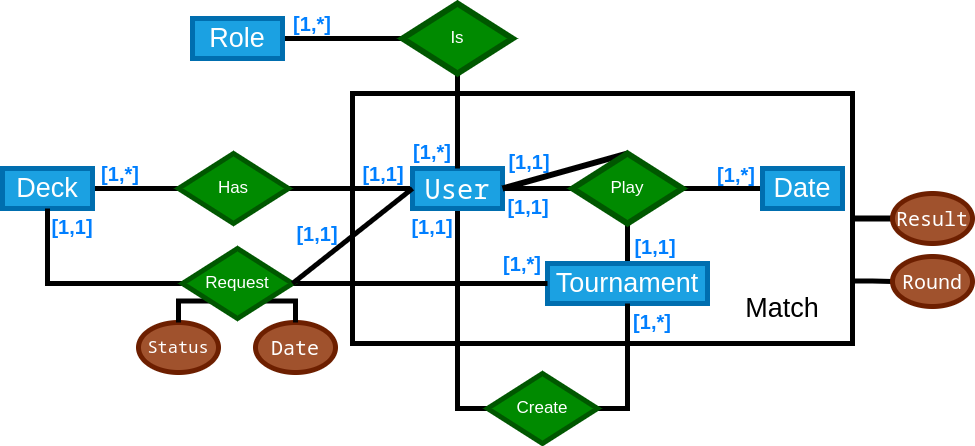
\includegraphics[width=1\textwidth]{merx.png}
  \caption{Esquema Relacional}
  \label{fig:etiqueta}
\end{figure}
\begin{figure}[h]
  \centering
  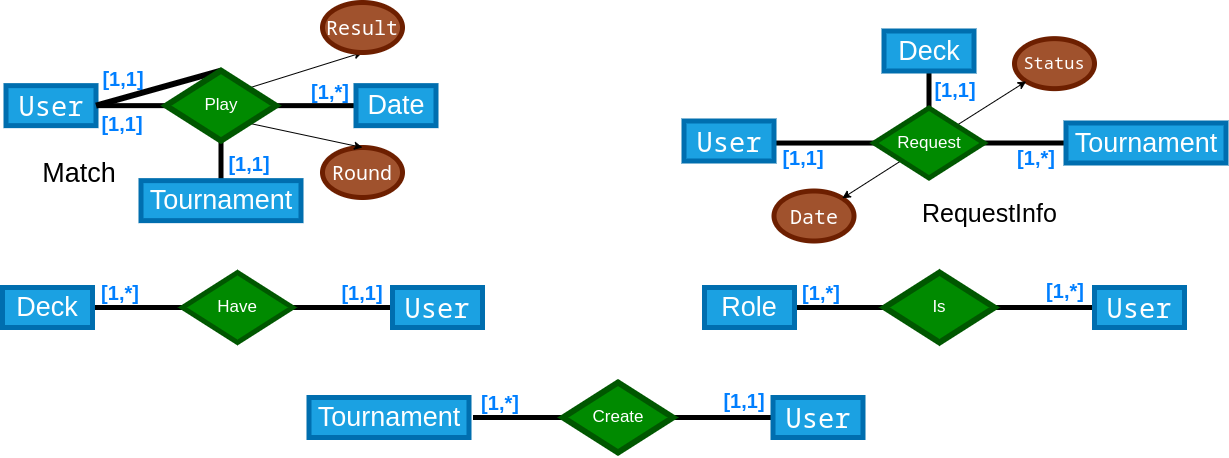
\includegraphics[width=1\textwidth]{relations.png}
  \caption{Esquema Relacional separado por relaciones}
  \label{fig:etiqueta}
\end{figure}
\newpage
\section{Valoraci\'on del dise\~no de la base de datos en cuanto a si es o no correcto:}

Sea el esquema relacional $R(U,F)$:

\textbf{Conjunto de Atributos}$(U)$
\begin{itemize}
  \item UserID, user$\_$name, township, province, phone $($optional$)$, address, DeckID, deck$\_$name, main$\_$deck$\_$sz, side$\_$deck$\_$sz, extra$\_$deck$\_$sz, archetype, TournamentID, tournament$\_$name, start$\_$date, location, RoleID, role$\_$name, date, result, round, status
\end{itemize}

\textbf{Dependencias Funcionales}$(F)$
\begin{description}
  \item[UserID] $\rightarrow$ [user$\_$name, township, province, phone (optional), address]
  \item[DeckID] $\rightarrow$ [RoleID]
  \item[DeckID] $\rightarrow$ [deck$\_$name, main$\_$deck$\_$sz, side$\_$deck$\_$sz, extra$\_$deck$\_$sz, archetype]
  \item[DeckID] $\rightarrow$ [UserID]
  \item[TournamentID] $\rightarrow$ [tournament$\_$name, start$\_$date, location]
  \item[RoleID] $\rightarrow$ [role$\_$name]
  \item[UserID, TournamentID] $\rightarrow$ [status, date]
  \item[UserID, TournamentID] $\rightarrow$ [DeckID]
  \item[UserID1, UserID2, TournamentID, date] $\rightarrow$ [IDUser1, IDUser2, IDTournament, Date]
  \item[UserID1, UserID2, TournamentID, date] $\rightarrow$ [Result, IDWinner, Round]
\end{description}

Sea $p = \{R1, R2, R3, R4, R5, R6\}$

$R1(U1,F1)$\\
\textbf{U1:}
\textbf{F1:}
\begin{description}
  \item[DeckID] $\rightarrow$ [deck$\_$name, main$\_$deck$\_$sz, side$\_$deck$\_$sz, extra$\_$deck$\_$sz, archetype]
  \item[UserID] $\rightarrow$ [RoleID]
\end{description}

$R2(U2,F2)$
\textbf{U2:}
\textbf{F2:}
\begin{description}
  \item[DeckID] $\rightarrow$ [deck$\_$name, main$\_$deck$\_$sz, side$\_$deck$\_$sz, extra$\_$deck$\_$sz, archetype]
  \item[DeckID] $\rightarrow$ [UserID]
\end{description}

$R3(U3,F3)$
\textbf{U3:}
\textbf{F3:}
\begin{description}
  \item[TournamentID] $\rightarrow$ [tournament$\_$name, start$\_$date, location]
\end{description}

$R4(U4,F4)$
\textbf{U4:}
\textbf{F4:}
\begin{description}
  \item[RoleID] $\rightarrow$ [role$\_$name]
\end{description}

$R5(U5,F5)$
\textbf{U5:}
\textbf{F5:}
\begin{description}
  \item[UserID, TournamentID] $\rightarrow$ [status, date]
  \item[UserID, TournamentID] $\rightarrow$ [DeckID]
\end{description}

$R6(U6,F6)$
\textbf{U6:}
\textbf{F6:}
\begin{description}
  \item[UserID1, UserID2, TournamentID, Date] $\rightarrow$ [UserID1, UserID2, TournamentID, date]
  \item[UserID1, UserID2, TournamentID, Date] $\rightarrow$ [result, round]
\end{description}

Dados un esquema relacional $R (U, F)$ y una descomposición $\rho = (R1, R2, \ldots, Rk)$, desde el punto de vista teórico, una base de datos relacional está correctamente diseñada o, simplemente, es un diseño correcto si se cumplen las tres propiedades siguientes: 
\begin{enumerate}
  \item Todos los esquemas relacionales $Rj (Uj, Fj)$ (j=1, ..., k) de la descomposición $\rho$ están en 3FN o una forma normal superior. 
  \item La descomposición $\rho$ satisface la propiedad de join sin pérdida de información (PLJ). 
  \item La descomposición $\rho$ satisface la propiedad de preservación de dependencias funcionales (PPDF).
\end{enumerate}

Mediante la aplicación del algoritmo pudimos hallar una descomposición $\rho$ que cumple con dos de las características de un diseño correcto. Ahora bien, la tercera condición (la satisfacción de PLJ) se puede comprobar fácilmente aplicando una de las consecuencias del lema que se presenta a continuación,

\textbf{Consecuencia} Si la llave X de $R (U, F)$ está contenida completamente en alguno de los esquemas relacionales de la descomposición, entonces, se puede afirmar directamente que $\rho$ es un diseño correcto 
En nuestro diserno se cumple con las tres propiedades requeridas las llaves candidatas (IDDeck, IDTournament) o (IDUser, IDTournament) y estas están completamente contenidas en $R5$.\\ \\

\begin{figure}[h]
  \centering
  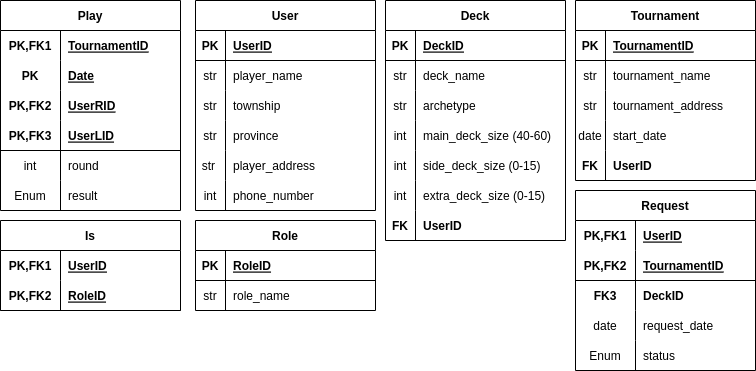
\includegraphics[width=1\textwidth]{table.png}
  \label{fig:etiqueta}
\end{figure}

\end{document}
 
